\documentclass[
 a4paper,twocolumn,showpacs,aip,groupedaddress,%
  eqsecnum,notitlepage,showkeys,cha,longbibliography,10pt
]{revtex4-1}
\usepackage[english]{babel}
\usepackage[utf8x]{inputenc}
\usepackage[T1]{fontenc}
\usepackage{amssymb}
\usepackage{amsmath,latexsym}
\usepackage{subcaption}
\usepackage{graphicx}
\usepackage{dcolumn}
\usepackage{tikz}
\usepackage{natbib}
\usepackage{float}
\usepackage[export]{adjustbox}
\usepackage{hyperref}
\usepackage{mathtools}
\usepackage{soul}
\DeclarePairedDelimiter\bra{\langle}{\rvert}
\DeclarePairedDelimiter\ket{\lvert}{\rangle}
\DeclarePairedDelimiterX\braket[2]{\langle}{\rangle}{#1 \delimsize\vert #2}

\newcommand*{\citen}[1]{%
  \begingroup
    \romannumeral-`\x % remove space at the beginning of \setcitestyle
    \setcitestyle{numbers}%
    \cite{#1}%
  \endgroup   
}

\usepackage[a4paper,top=1.8cm,bottom=1.8cm,left=1.5cm,right=1.5cm]{geometry}
\usepackage[skip=5pt, font=scriptsize, labelfont=bf, justification=raggedright]{caption}

\usepackage{titlesec}

\titlespacing\section{0pt}{12pt plus 4pt minus 2pt}{0pt plus 2pt minus 2pt}

\graphicspath{ {Images/} }

\begin{document}

\title{\LARGE{Prospects for Quantum Computing with Quantum Dots}}

\author{Lindsey Keary}
\affiliation{ 
Student Number : 17099595, l.keary.17@ucl.ac.uk, University College London
}
\date{\today}\ 


\input{abstract}


\maketitle

% \input{leadpara}

\section{\label{sec:level1}Introduction}
Present day computers emerged from the principles of "the computing machine model", now referred to as the Turing machine, devised by Turing in 1936 [\citen{Turing1937OnEntscheidungsproblem,Nielsen2010QuantumInformation}]. The impactful development of the first integrated circuit (IC) in 1958 provided a cheap and fast operated basic chip element for building the computer mainboard [\citen{Arns1998TheTransistor}]. Moore's trend predictions since 1965 of the population increase by reduction in the size of transistors on a IC chip, have held accurate for the past three decades [\citen{Moore1965CramingCircuits,GordonE.Moore1975ProgressElectronics}]. However, continuing to increase processing power by the scale down method is reaching the fundamental limit of the transistor size resulting in quantum effects of electrons dominating circuit operation. Quantum computing is being investigated as an alternative speed-up method to solve problems which cannot be efficiently solved using classical computation [\citen{Waldrop2016TheLaw,Fox2006QuantumIntroduction}]. Active areas of research of many systems include: neutral atoms, trapped ions, superconducting circuits and photons assess the feasibility of realising universal quantum computation by providing the basic unit for quantum computing known as the qubit [\citen{Saffman2016QuantumChallenges,Brown2016Co-designingIons,Gambetta2017BuildingSystem,Milburn2009PhotonsQubits}].  


Quantum dots (QDs) are nanoscale structures which have potential to be implemented as a qubits due to their ability to confine and address single electrons using gate electrodes [\citen{Imamoglu2003AreComputation}]. Despite self-assembled QDs [\citen{Warburton2013SingleDots}] also being a promising candidate source of qubits, where the system is controlled optically, this report will focus on the advancements of gate-controlled quantum dots exclusively. The most matured spin or charge state encoding of QDs has been achieved using GaAs/AlGaAs heterostructures, where the coherence time is limited by fluctuations in environment. Therefore, fabrication of QDs using materials which have a low abundance of nuclear spin, such as carbon, C and silicon, Si reduces the spin state decoherence route [\citen{Schroer2008TimeOut}]. This report reviews recent developments of quantum dot qubit implementation where the DiVincenzo criteria [\citen{Divincenzo2000TheComputation}] provides a means to assess the future prospects of QDs satisfying the requirements to realise a quantum computer.



\section{Theoretical Background}
Fabrication techniques such as electron beam lithography (EBL) are used to produce the GaAs/AlGaAs heterostructure. The heterostructure enables a small number of free electrons, with the DeBroglie wavelengths similar to the QD size, to be confined in a quantum well \citen{BoscoQuantumEffect}. The electrons between the GaAs and AlGaAs semi-conducting surfaces act as a 2-dimensional electron gas (2DEG) [\citen{Ihn2009SemiconductorNanostructures,Kouwenhoven1997IntroductionTransport}]. Etching gate electrodes on the surface of the GaAs layer enables controlled confinement of the electrons to 3-dimensions. Therefore these artificial atoms result in electrons occupying discrete energy levels, observed at low temperatures, which follow atomic physics rules. Therefore, quantum dot devices are contained within a dilution refrigerator where the electrons are kept at $\approx100$ mK temperatures during experiments [\citen{Petta2004ManipulationDot}]. 

The Coulomb repulsion between electrons must be overcome to add an additional electron to the dot. The electro-chemical potential is the energy difference between the single dot ground state containing $N$ and $N+1$ electrons: 

\begin{equation}
\label{eq:interactionham0}
\mu (N) = -\frac{E_{C}}{\left | e \right |}(C_{S}V_{S}+C_{D}V_{D}+C_{G}V_{G})+E_{N}, 
\end{equation}

where charging energy to cross the junction into the dot is $E_{C}=\frac{e^{2}}{C}$. The total capacitance $C$ is the sum of the capacitance of the source, drain and gate electrodes which are $C_{S}, C_{D}$, and $C_{G}$, respectively. Similarly for the applied electron voltages, $V_{S}, V_{D}$ and $V_{G}$ as shown in Fig. (\ref{fig:QDaa}). The chemical potential energy of Nth additional electron is $E_{N}$. The additional energy is thus given as: 

\begin{equation}
\label{eq:interactionham0}
E_{add}(N)=\mu(N+1)-\mu(N)=E_{C}+E_{N+1}-E_{N},
\end{equation}

where spin filling resulting from the Pauli exclusion principle dictates the value of $E_{N+1}-E_{N}$ being zero or nonzero [\citen{Hanson2007SpinsDots}]. 
 
\begin{figure}[t]
\centering
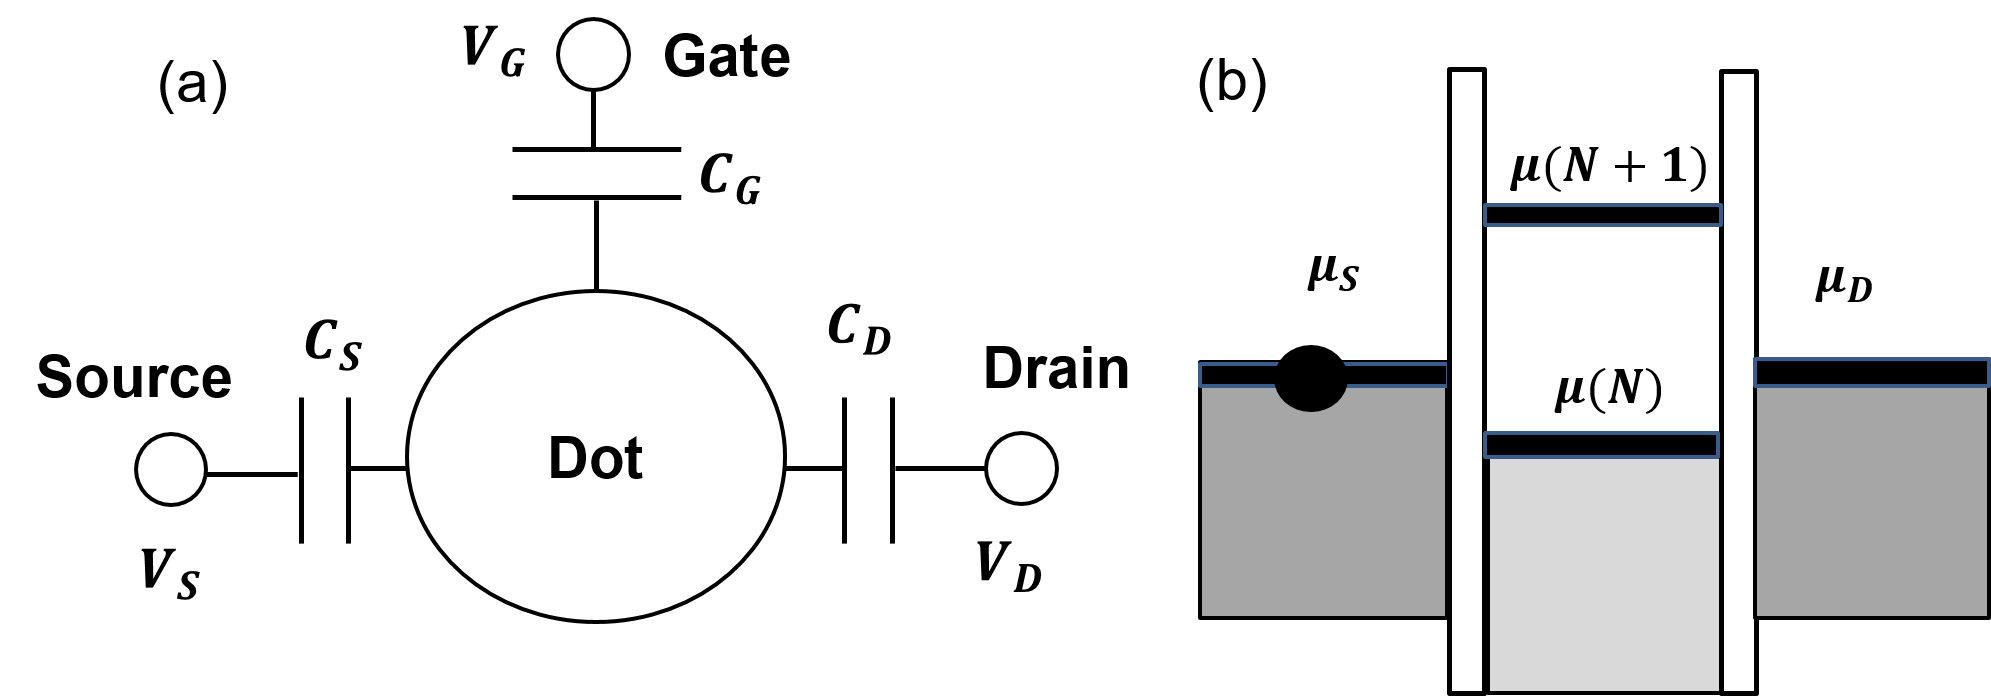
\includegraphics[height=0.18\textwidth,keepaspectratio]{QDaa}
\caption{\label{fig:QDaa}(a) Single QD schematic showing electrode connections. (b) Energy level diagram with the Coulomb blockade condition satisfied.}
\end{figure} 

Controlling of voltage of the electrodes allows electrons to tunnel into the QD. The Coulomb blockade refers to the case where $\mu_{S} \geq \mu(N) \geq \mu_{D}$ and the QD electron number is constant. Extension of this derivation to include double QDs is given in Ref. [\citen{vanderWiel2002ElectronDots}] where each dot has a individual plunger gate electrode. An additional gate electrode of voltage $V_{M}$ separates the dots. Double quantum dots enable encoding of the charge or spin degree of freedom of the qubit. 
  

  



\subsection{Qubit Realisation, Initialisation and Measurement}
\subsubsection{Charge Qubit}
In lateral double QDs an electron confined can be approximately described as being in the left $\ket{L}=(1,0)$ or right $\ket{R}=(0,1)$ spatial state. The two charge states produce the charge qubit. In the weak coupling regime the electron is initially localised to a charge state however the electron becomes delocalised with equal probability of being in either charge state when the tunnel coupling strength is increased [\citen{OosterKamp1998MicrowaveMolecule}]. The voltage $V_{M}$ of the electrode between the QDs controls the tunnel coupling potential-wells. The tunnel coupling energy, $2\Delta$ produces the charge state anti-crossing in the strong coupling regime as shown in Fig. (\ref{fig:QD1}). The Hamiltonian describing the two-level charge qubit is $H=\frac{1}{2}\epsilon \sigma_{z}+\Delta\sigma_{x}$, where the gate electrodes control the detuning, $\epsilon$ between qubit energy states. The energy splitting is given as $\Omega(\epsilon)=\sqrt{\epsilon^{2}+(2\Delta)^{2}}/\hbar$ [\citen{Hayashi2003CoherentDot}]. Demonstration of manipulation of the charge double QD using microwave pulses resonant with $\Omega$ and control of the tunneling coupling enables mapping of the charge stability diagram for the charge states [\citen{Petta2004ManipulationDot}]. 

\begin{figure}[b]
\centering
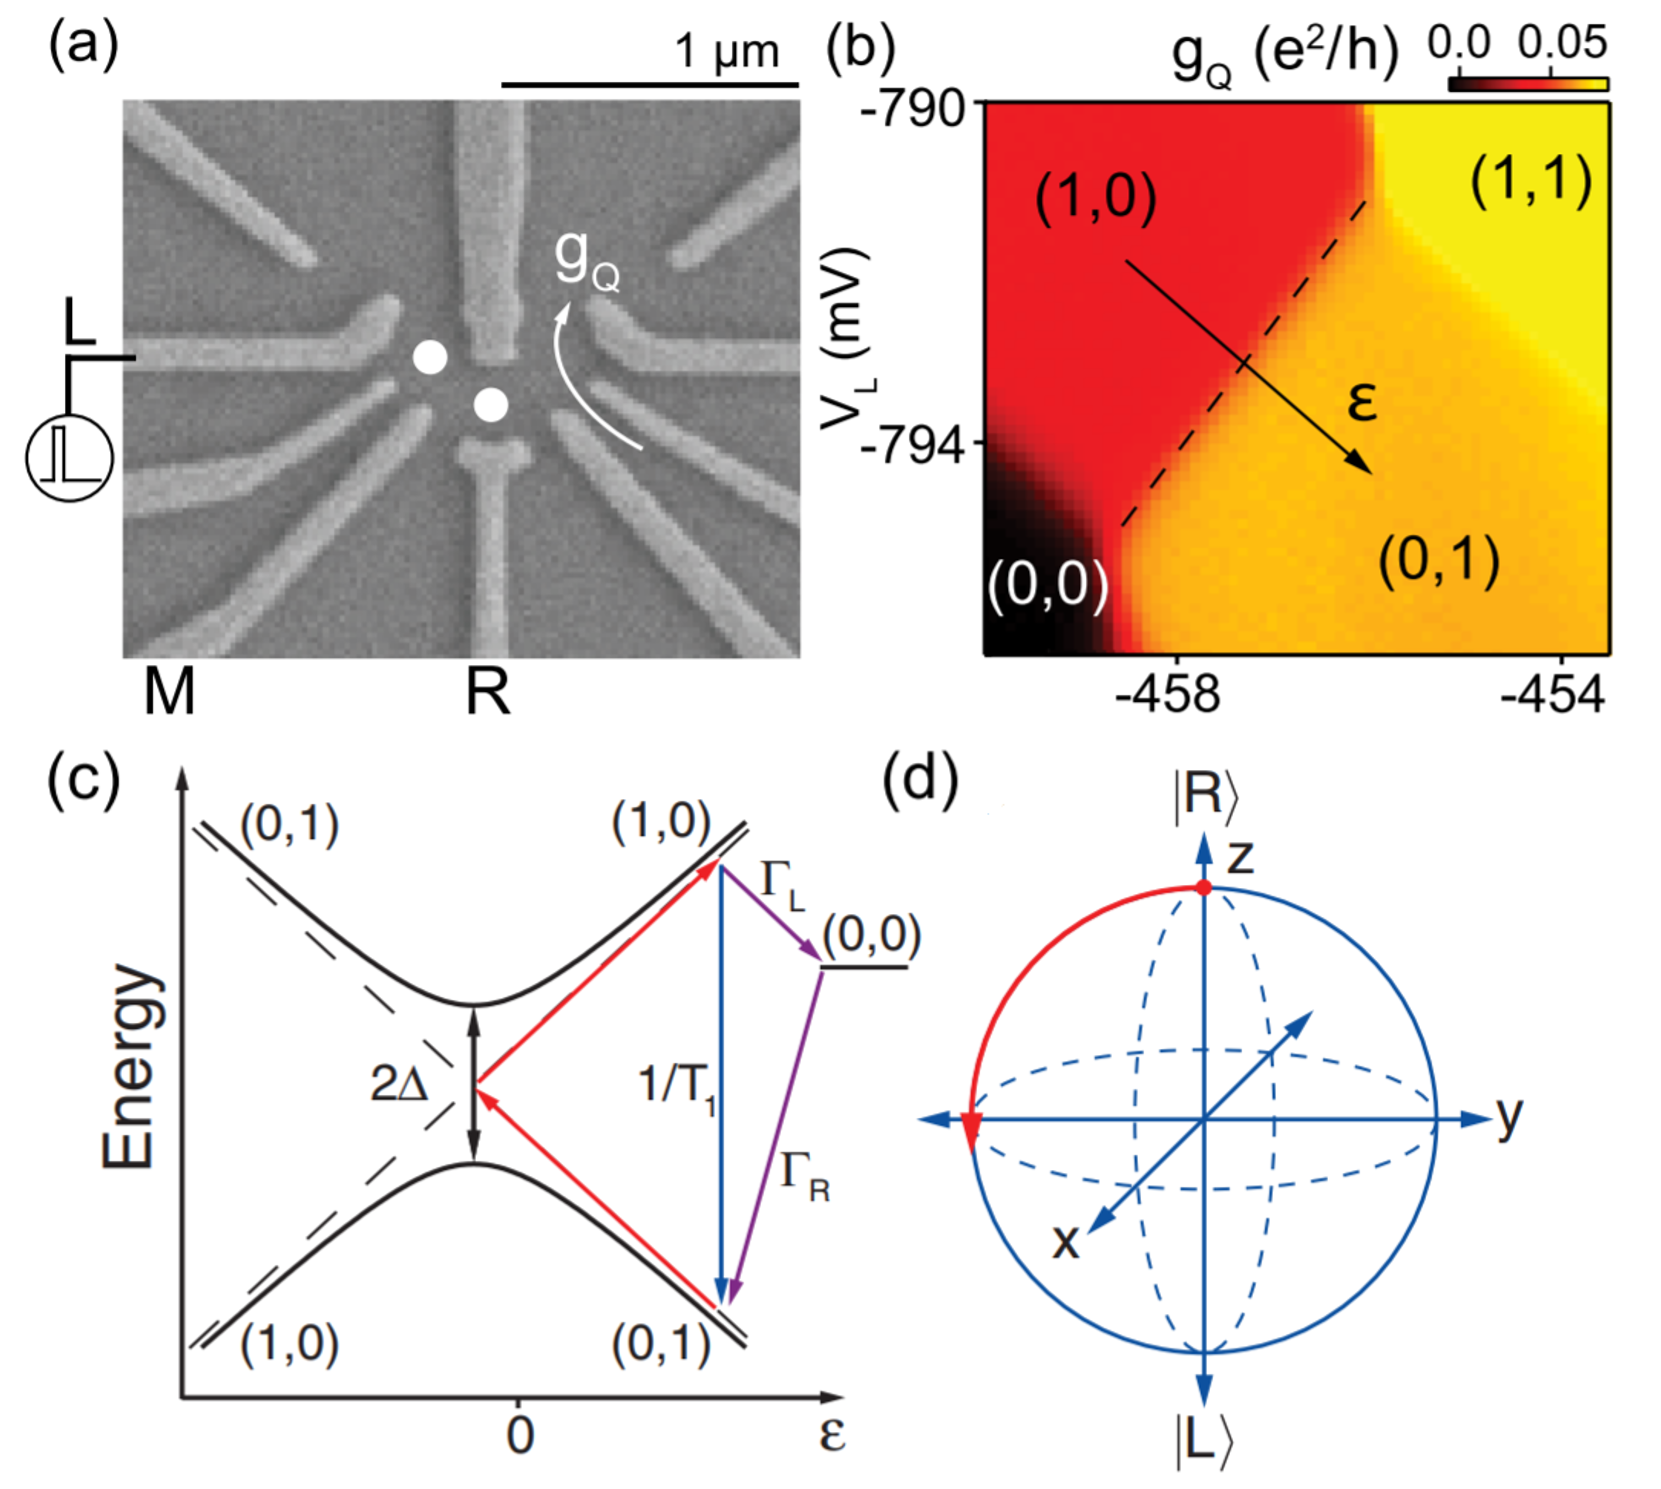
\includegraphics[height=0.4\textwidth,keepaspectratio]{QD1}
\caption{\label{fig:QD1}(a) Scanning electron microscope image of the lateral double QD device where a QPC contact measuring the conductance is labeled. (b) The charge stability diagram obtained using a QPC sensor. (c) Energy level diagram with the pulse sequence shown in red. The state $\ket{R}$ is initialised, then adiabatically pumping to $\epsilon=0$ prepares a the block sphere rotation in (d). Then returning to $\epsilon >> 2\Delta$ produces the rotation to $\ket{L}$. The decay rate of other charge states is shown in blue and purple \citep{Petersson2010QuantumQubit}.}
\end{figure}

Charge sensing is used extensively in recent quantum dot studies where the quantised steps of the conductance $G$ across a quantum point contact (QPC) is measured as $V_{G}$ is swept for each dot.The QPC is fabricated by 2DEG depletion of the heterostructure between two narrowly spaced electrodes [\citen{VanWees1988QuantizedGas}]. $X$-axis Bloch sphere rotations are completed in Ref.[\citen{Petersson2010QuantumQubit}] by adiabatically applying drain voltage pulses in the sequence shown in Fig. (\ref{fig:QD1}c) within the charge state relaxation time $T_{1} \approx 10$ ns. Observing the decay of coherent oscillations obtains the maximal coherence time $T_{2}=7$ ns when operated at $\epsilon=0$ to remove the sensitivity to first order charge noise caused by gate charge fluctuations. Similarly the sweet point occurs for superconducting charge qubits [\citen{Han2001Time-ResolvedJunction}]. 

Therefore fast operation makes charge QDs a promising elementary component for quantum computing which is currently limited by the decoherence due to charge noise [\citen{Koh2013High-fidelityQubits.}]. Universal single qubit gate rotations are performed on a Si/SiGe double QD ($T_{1}=23.5$ ns) in Ref. [\citen{Kim2015Microwave-drivenQubit}] . This was achieved by adiabatically pumping to a superposition state from a charge state as shown in Fig. (\ref{fig:QD1}c) however now the superposition states $\ket{0}=(1/\sqrt{2})(\ket{L}+\ket{R})$ and $\ket{1}=(1/\sqrt{2})(\ket{L}-\ket{R})$ produce the Z-axis Bloch states. Then applying two ac resonant $X_{\pi/2}$ pulses, with individual maximum rotation time of 125 ps, and a time evolution $t_{e}$ between them enables Z-axis rotations. Changing the phase of the second microwave pulse illustrates the freedom to implement arbitrary plane rotations.  
   

\subsubsection{Spin Qubit}

\begin{figure}[b]
\centering
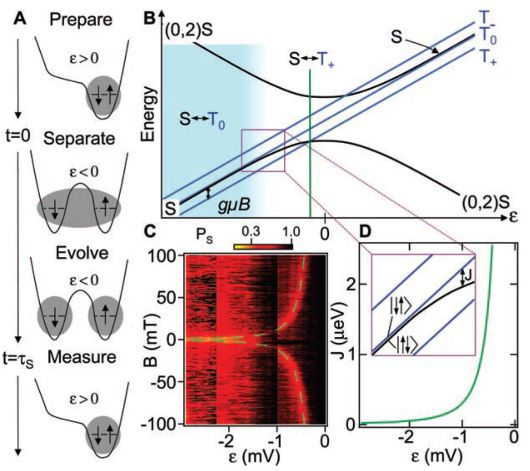
\includegraphics[height=0.4\textwidth,keepaspectratio]{QD2}
\caption{\label{fig:QD2} (a) The qubit is initialised to the S(0,2) state then it is pulsed with $\epsilon < 0$ into the S(1,1) state which evolves for some time $\tau_{s}$ and can mix with the $T_{0}$ state. Projection back into the S(0,2) state allows charge occupancy readout using the QPC detector since the transition from $T(1,1) \rightarrow T(0,2)$ is not accessible. (b) The energy level diagram showing the singlet and triplet states in the presence of a magnetic field after $\tau_{s} =200$ ns. (c) Probability of S(0,2) detection as a function of $\epsilon$ and $B$. (d) Exchange detuning as a function of $\epsilon$ where $S$ and $T_{0}$ are split by $J(\epsilon)$  \citep{Petta2005CoherentDots}.}
\end{figure}

The QD spin states arise due to the intrinsic spin property of an electron. The electron spin is orientated parallel or antiparallel to an applied magnetic field, $\vec{B}$. A two-electron single QD can be used to form a spin qubit. Single-shot readout of the qubit state is demonstrated in Ref. [\citen{Elzerman2004Single-shotDot}] by utilising a QPC sensor and the Zeeman energy splitting between the spin-up ($\ket{\uparrow}$) and spin-down ($\ket{\downarrow}$) states. However, the gate control of tunnel coupling between dots is an advantage of using double QDs where the lowest energy levels for two-electrons are the singlet $\ket{S}=\frac{1}{\sqrt{2}}(\ket{\uparrow \downarrow}-\ket{\downarrow \uparrow})$  ($s=0$, $m_{s}$=0) and triplet $\ket{T_{+}}=\ket{\uparrow \uparrow}$, $\ket{T_{0}}=\frac{1}{\sqrt{2}}(\ket{\uparrow \downarrow}+\ket{\downarrow \uparrow})$, $\ket{T_{-}}=\ket{\downarrow \downarrow}$  ($s=1$, $m_{s}=-1,0,1$) states [\citen{Viennot2016TowardsDots,Wesslen2017ConfinementRelaxation}]. Conversion to charge sensing is enabled due to the Spin blockade of the transition to the higher energy state triplet T(0,2) while transitions between the states the S(1,1) S(0,2) and T(1,1) are energetically accessible [\citen{Hao2014ElectronDot}]. 

In Fig. (\ref{fig:QD2}a) the control steps of the spin states are outlined, for the GaAs/AlGaAs two-particle double QD, where the measured time-ensemble-averaged dephasing time $T2^{*}$ was 10 ns [\citen{Petta2005CoherentDots}]. The energy level diagram for the spin states is given in Fig. (\ref{fig:QD2}b) where the $S$ charge states form an anti-crossing and the triplet states are degenerate when $\vec{B} \neq 0$. The splitting energy $J(\epsilon)=g^{*}\mu_{B}B$ between the states $S$ and $T_{0}$ is a function of $\epsilon$ where $\mu_{B}$ is the Bohr magneton and $g^{*}$ is the g-factor of the host material. The resulting eigenstates are $\ket{\uparrow \downarrow}$ and $\ket{\downarrow \uparrow}$. The $S-T_{0}$ Hamiltonian is give as:


\begin{equation}
\label{eq:interactionham0}
H=\begin{pmatrix}
J(\epsilon) &  \delta B^{z}_{nuc}\\ 
\delta B^{z}_{nuc} & 0
\end{pmatrix}.
\end{equation}

\begin{figure}[b]
\centering
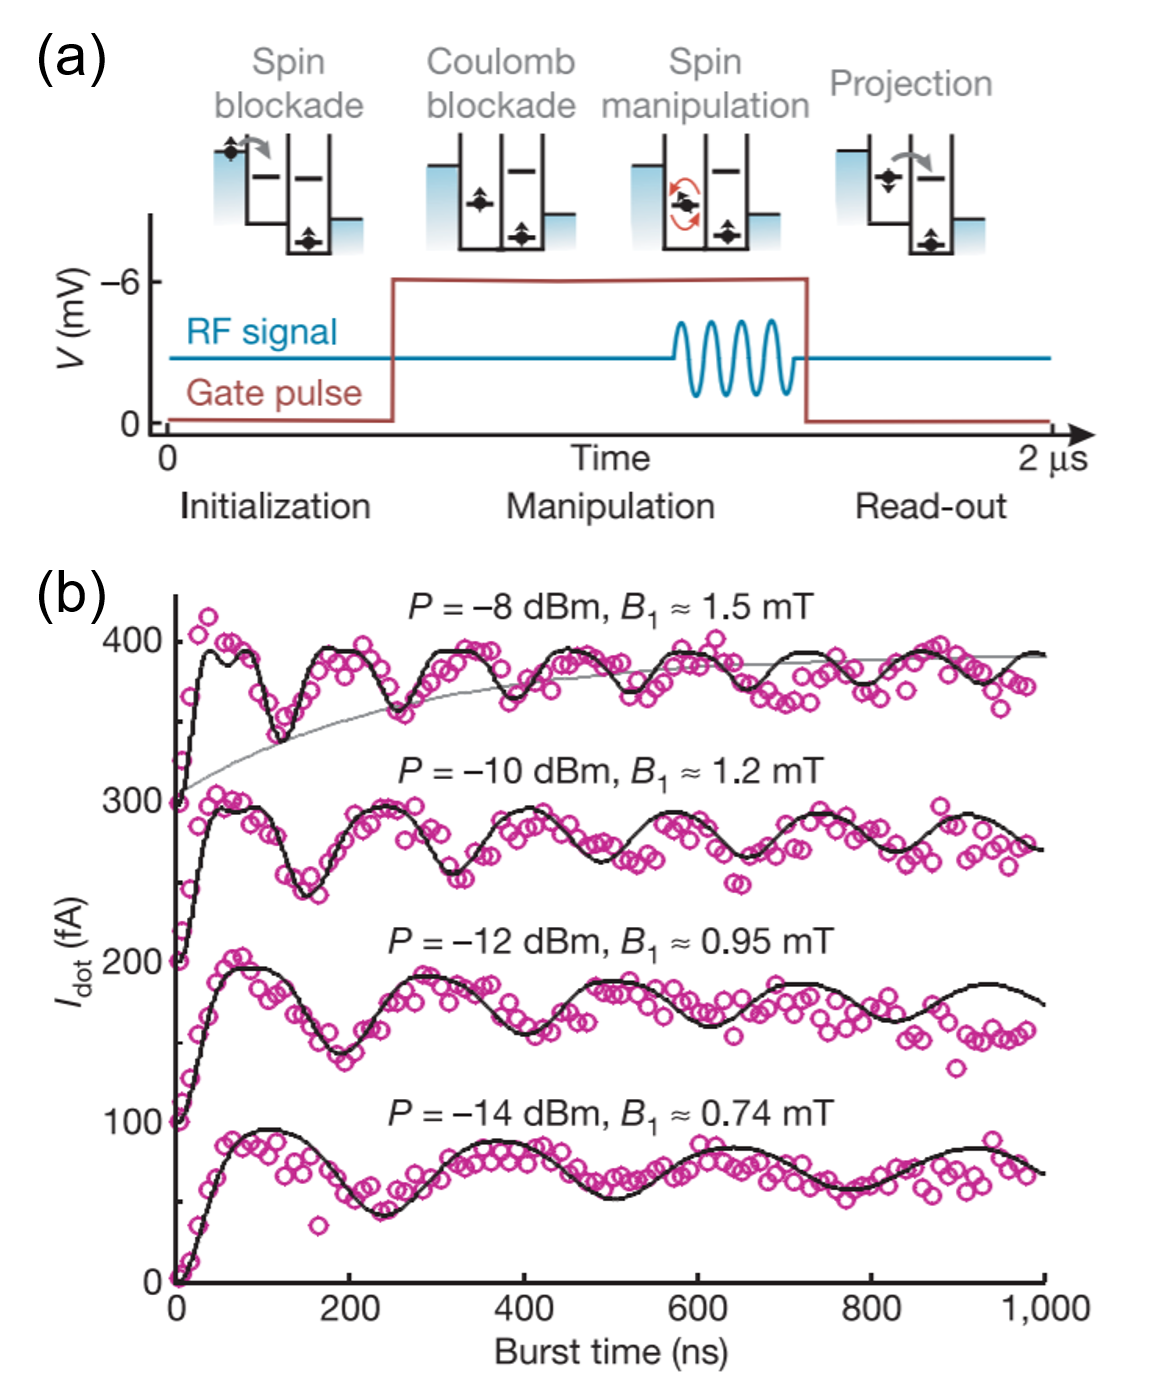
\includegraphics[height=0.45\textwidth,keepaspectratio]{QDe}
\caption{\label{fig:QDe} (a) The control cycle for single spin coherent oscillation where the manipulation used the ESR technique by applying to a rf-pulse to the electrode of the left QD. (b) The coherent Rabi oscillation measured for various applied rf power \citep{Koppens2006DrivenDot}.}
\end{figure}


The slowly evolving Overhauser field has a gradient across the dots which is given by $\Delta B^{z}_{nuc}$. The Overhauser field $B^{z}_{nuc}$ increases the total external magnetic field and arises due to the hyperfine interaction between magnetic moment of $1\approx 10^{6}$ nuclei in a QD and the electrons [\citen{Chekhovich2013HyperfinePolarization,LandiDeglInnocenti2014AtomicProcesses}]. Therefore dephasing occurs due to induced coupling of $S$ and $T_{0}$ (and similarly for $S$ $T_{+}$). Consequently the rate of pulsing the detuning from the S(0,2) state around $\epsilon < 0$ enables transition into $\ket{\uparrow \downarrow}$ which is used to produce the SWAP gate. Furthermore in Ref. [\citen{Petta2005CoherentDots}] the echo sequence detailed achieves the coherence time of 1 $\mu$s by correcting for evolution from the $S$ to $T_{0}$ caused by dephasing. Fluctuations of the nuclear field $\delta B^{z}_{nuc}$ arise due to interactions between the randomly orientated nuclear spins and results in decoherence  [\citen{Khaetskii2002ElectronNuclei}]. Coherent oscillations > 1 $\mu$s in a two-particle double QD are measured by the current induced by the electron spin resonance (ESR) manipulation of a single electron \citep{Koppens2006DrivenDot}. The control cycle is shown in Fig. (\ref{fig:QDe}b). ESR is a spectroscopy technique which enables the transition from one spin orientation to the other in spin-1/2 particles by the action of a perpendicular high-frequency magnetic-field [\citen{Loubser1978ElectronDiamond}]. Initialisation prepares electrons in Spin Blockade with parallel spins where Coulomb blockade additionally increases $\mu_{R}$ above $\mu_{L}$ such that independent of the left electron spin rotation the S(0,2) state is inaccessible as shown in Fig. (\ref{fig:QDe}a). Thus intra-dot tunneling decoherence is removed and readout is detected by lifting the Coulomb blockade between dots.  


\subsection{Increasing Coherence Time}
Charge QDs are a promising elementary component for quantum computing due to fast gate control but are limited by the decoherence due to 1/frequency charge noise [\citen{Koh2013High-fidelityQubits.,Petersson2010QuantumQubit}]. Operation at the $\epsilon=0$ sweet spot and Hahn-echo decoupling achieve moderate coherence times of $T_{2}^{*} \approx 1.3$ ns [\citen{Kim2015Microwave-drivenQubit}]. The avenues available to improve the coherence time of spin qubits are extensive. The Carr–Purcell–Meiboom–Gill (CPMG) echo sequence shown in Fig. (\ref{fig:QDcpmg}b) is applied to spin qubits to decouple the electrons in the S(1,1) state from slow fluctuations of $\Delta B_{nuc}$ allowing for coherence times > 200 $\mu$s [\citen{Bluhm2011DephasingS}]. This scheme is similar to the Hahn echo sequence except it applies a series of $\pi$-pulses to produce X-gate rotations between the $S$ and $T_{0}$ states. 

This report has focused on GaAs/AlGaAs heterostructure as the host material due it being the workhorse of double QD research. However, $^{29}$Si is the only isotope in Si with a nuclear spin, thus Si and isotropically purified $^{28}$Si are regarded as promising lattice materials [\citen{Tyryshkin2006CoherenceSilicon,Ken-ichiroTakyu2003TheSecon}]. However, it does not come without it's own challenges including the difficulty to implement state manipulation due to 6-fold valley degeneracy. This can be reduced to 2 when Si is under strain and results in state mixing decoherence [\citen{Boykin2004ValleyWells,Goswami2006ControllableDevices}]. Additionally an important aspect when building a quantum computer is having high fidelity single-shot readout to enable dynamic error correction [\citen{Urdampilleta2017TowardsDetector}].

Manipulation and single-shot readout is demonstrated in Ref. [\citen{Barthel2009RapidQubit}] where the degeneracy is lifted for the 2-fold valley for acutely confined electrons of doped phosphorus, P atoms. The Si single electron transistor which has equivalent gate electrode configuration to a single quantum dot completes charge sensing in addition to tunnel coupling to P. An electron is transferred from the SET to donor with a random spin state. Readout is enabled when the condition $\mu_{\downarrow}<\mu_{SET}<\mu_{\uparrow}$ by measurement of the current induced by $\ket{\uparrow}$ tunneling into the SET. The fidelity of this system is comparable to the >90 $\%$ fidelity obtained for single-shot readout of the GaAs double QD using rf-QPC detection [\citen{Barthel2009RapidQubit}]. 

\begin{figure}[b]
\centering
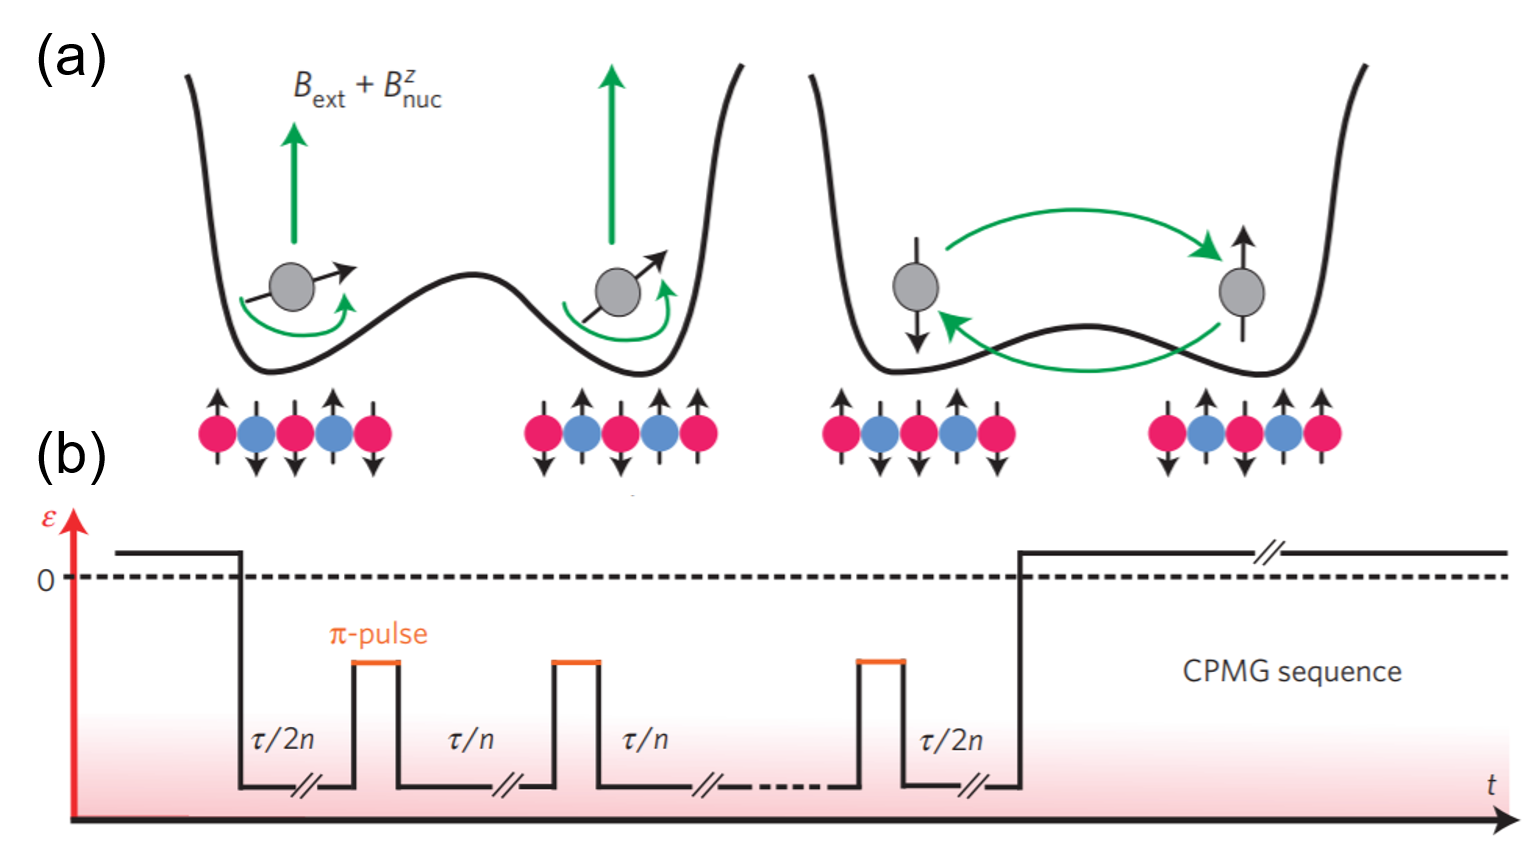
\includegraphics[height=0.25\textwidth,keepaspectratio]{QDcpmg}
\caption{\label{fig:QDcpmg} (a) The double-potential well representation of the prepared S(1,1) state where the hyperfine field produces rotations between the $S$ and $T_{0}$ states (left). Therefore by increasing intra-dot coupling results the spin-exchange interaction (right). (b) The CPMG scheme applies $\pi$ pulses to continually switch the spin states and effectively decouple from the hyperfine field \citep{Bluhm2011DephasingS}.}
\end{figure}

\begin{figure}[t]
\centering
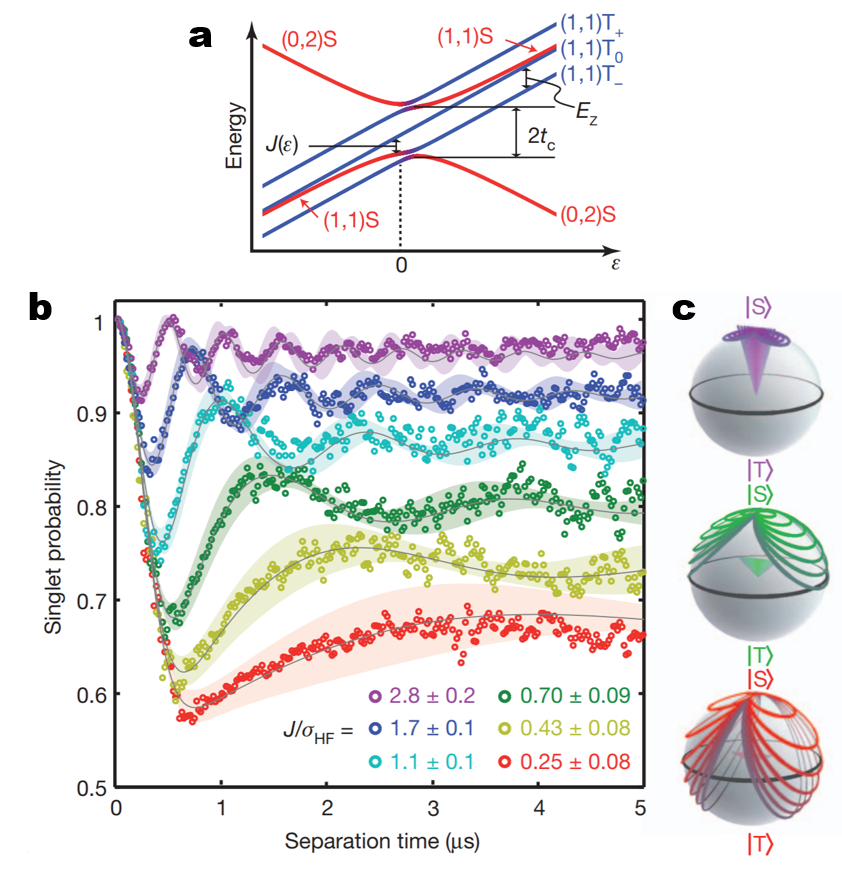
\includegraphics[height=0.4\textwidth,keepaspectratio]{QD31}
\caption{\label{fig:QD31}(a) Energy level diagram for the Si/SiGe double QD. (b) Dephasing of coherent oscillations where (b) illustrates the Bloch sphere representation of the resulting rotations \citep{Maune2012CoherentDot}.}
\end{figure}

\begin{figure}[b]
\centering
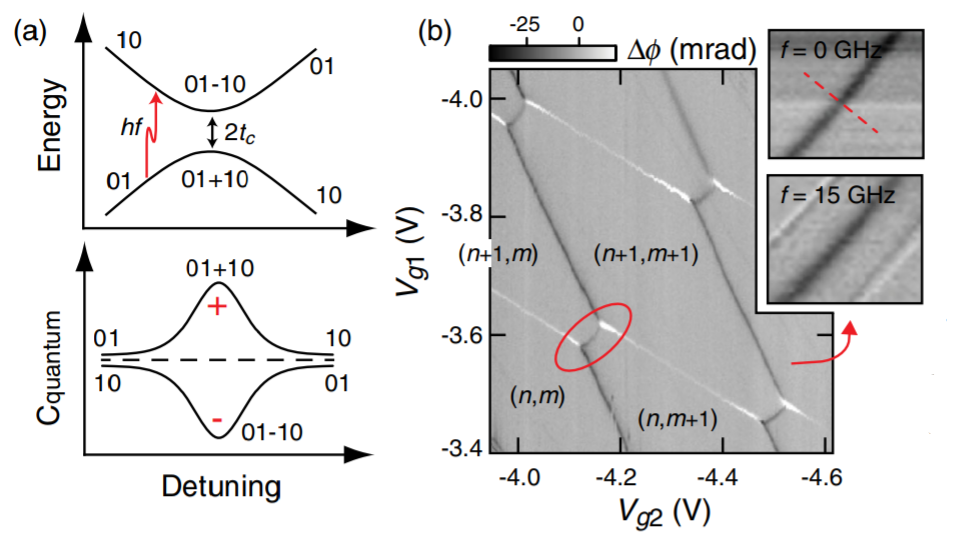
\includegraphics[height=0.27\textwidth,keepaspectratio]{QDl}
\caption{\label{fig:QDl}(a) Energy band diagram (top) and corresponding quantum capacitance (bottom) as a function of level detuning  for a double quantum dot with one electron. (b) Charge stability diagram measured by the phase response of a carbon nanotube double quantum dot coupled to an electrical resonator \citep{Penfold-Fitch2017MicrowaveQubit}.}
\end{figure}

Coherent oscillations of the superposition between $S$ and $T_{0}$ states in a Si host material shown in Fig. (\ref{fig:QD31}b) are pulsed by controlling $J$. The energy level diagram for the Si/SiGe double QD is given in Fig. (\ref{fig:QD31}a) for the singlet and triplet states where the magnitude of $J$ for $S-T_{0}$ is shown to be a function of $\epsilon$. Dephasing due to $B_{nuc}$ from the low abundance of nuclear spins and charge noise fluctations limits $T_2^{*}$ to 360 ns [\citen{Maune2012CoherentDot}]. The Bloch sphere representation of the dephasing resulting in the decay of the Rabi oscillations is shown in Fig. (\ref{fig:QD31}c). Another technique to create fast coherent oscillations of $S-T_{-}$ and $S-T_{0}$ states in Si uses a magnet positioned closer to one quantum dot where the maximum $T_{2}^{*}$ presented was 1.7 µs [\citen{Wu2014Two-axisMicromagnet.}]. This artificially creates a static $\delta B^{z}_{nuc}$ between the dots which is present but fluctuates naturally in host materials with nuclear spin [\citen{Petta2005CoherentDots}]. Due to the extension of the coherence time in Si QD systems, 100 Controlled-Not (CNOT) gates are performed in Ref. [\citen{Veldhorst2015ASilicon}] each with a operation time of 100 ns. The isotropically purified $^{28}$Si double QD device is controlled using the ESR spectroscopy and each dot represents a single qubit which is individually manipulated using the Stark effect. CNOT gates in addition to single qubit gates enable the formation of the universal gate set required for quantum computing [\citen{Nielsen2010QuantumInformation}]. 



The 1\% abundance of $^{13}$C in naturally occurring C provides a weak hyperfine interaction and is therefore considered promising for fabrication of spin quantum dots with long coherence times [\citen{Fischer2009HyperfineDots}]. Lateral Graphene, carbon nanotubes (CNT) and Buckminsterfullerene are examples of C quantum dots where the degree of inherent electron confinement depends on the fullerene structure [\citen{Alvarez-Diduk2017PaperReadout,Tans1997IndividualWires,Lu2011TransformingDots}]. In Ref. [\citen{Penfold-Fitch2017MicrowaveQubit}] a CNT is used to form quantum dots on a Si/SiO$_{2}$ heterostructure. Manipulation is completed through coupling the charge qubits to a resonant circuit and measuring the phase of the reflected rf signal output enables charge state detection. The phase is dependent on quantum capacitance which has a level structure shown in Fig. (\ref{fig:QDl}a). Therefore, readout is completed whilst operating at the charge noise sweet stop. The sensitivity of the measurement provides the sharp mapping of the charge stability diagram as shown in Fig. (\ref{fig:QDl}) which highlights the capability of this sensing technique.   



\section{Outlook}
Currently it appears that gate-defined QD fabrication using naturally occuring or istopically purified Si, and C, are the most promising candidates to produce long-lived qubits. QDs fabricated in GaAs/AlGaAs heterostructures can achieve coherence times of > 1 $\mu$s but are ultimately limited by fluctations of $B^{z}_{nuc}$. However, the continued research of GaAs quantum dots is valuable due to the the understanding gained of techniques to implement coherent manipulate of various spin qubits and produce sequences to reduce qubit decoherence effects [\citen{Maune2012CoherentDot,Wu2014Two-axisMicromagnet.,Veldhorst2015ASilicon}]. For example the coherence time achieved in Ref. [\citen{Veldhorst2015ASilicon}] of $T_2^{*} =120 \mu$s for one Si spin qubit could be further improved by correcting the charge noise, from exchange coupling to the other qubit, through the use of the CPMG scheme. 

In addition, further investigation of charge qubit readout is required due to charge noise coupling to the system in schemes which rely heavily on spin-charge conversion [\citen{Divincenzo2000TheComputation,Petta2005CoherentDots,Penfold-Fitch2017MicrowaveQubit}]. Future QD research steps with the goal to satisfy all DiVincenzo criteria include: dephasing reduction techniques for spin and charge qubits in lattice materials with low nuclear-spin coupling, increased fidelity of single-shot readout, investigation of hybrid quantum systems involving quantum dots (eg. coupled to superconducting resonators [\citen{Petersson2012CircuitQubit}]) and schemes involving increased numbers of qubits. 



 
 



\input{acknowledgements}


\bibliographystyle{ieeetr}

\bibliography{main}

\end{document}